% This work is licensed under the Creative Commons
% Attribution-NonCommercial-ShareAlike 4.0 International License. To view a copy
% of this license, visit http://creativecommons.org/licenses/by-nc-sa/4.0/ or
% send a letter to Creative Commons, PO Box 1866, Mountain View, CA 94042, USA.

\newcommand{\directoryPrefix}{../latex/} % Je nach Ordnertiefe muss dieser Command angepasst werden. Bei Fragen mich anschreiben.
\input{\directoryPrefix templates}
\TemplateSummary{Willi Sontopski}{PDENM}

\begin{document}
	\section{Sobolev-Räume}
	
	$\Omega\subseteq\R^d$ offen und beschränkt.
	Aus dem Divergenz-Satz von Gauß folgt die erste Greensche Formel:
	\begin{align}\label{eqGreen}
		\int\limits_\Omega\nabla u\cdot\nabla v\d x
		=\int\limits_{\partial\Omega}v\cdot\nabla u\cdot n\d S-\int\limits_\Omega v\cdot\Delta u\d x\quad\mit\quad
		\div(\nabla u)=\laplace u=\sum\limits_{k=1}^n\frac{\partial^2 f}{\partial x_k^2}
	\end{align}
	$D^\alpha\varphi$ \textbf{$\alpha$-te schwache Ableitung} von $\varphi\in L^1(\Omega)\gdw
	%\begin{align*}
		\forall v\in C_0^\infty(\Omega):\int\limits_\Omega\varphi\cdot \underbrace{D^\alpha v}_{\overset{\alpha=1}=v'}\d x
		=\underbrace{(-1)^{|\alpha|}}_{\overset{\alpha=1}{=}-1}\cdot\int\limits_\Omega D^\alpha\varphi\cdot v\d x$
	%\end{align*}
	eindeutig bestimmt, stimmt mit klassischer Ableitung überein, $|x|$ ist schwach diffbar
	\begin{align*}
		W^{k,p}(\Omega)
		&:=\Big\lbrace\varphi\in L^p(\Omega):D^\alpha\varphi\text{ (schwache Abl.) existiert und }D^\alpha\varphi\in L^p(\Omega)~\forall|\alpha|\leq k\Big\rbrace
		\quad k\in\N_0,p\in[1,\infty)\\
		\Vert\varphi\Vert_{k,p,\Omega}
		&:=\left(\sum\limits_{|\alpha|\leq k}\left\Vert D^\alpha\varphi\right\Vert^p_{L^p}\right)^{\frac{1}{p}}
		=\left(\sum\limits_{|\alpha|\leq k}\int\limits_\Omega\left| D^\alpha\varphi(x)\right|^p\d x\right)^{\frac{1}{p}};~\Big(W^{k,p}(\Omega),\Vert\cdot\Vert_{k,p,\Omega}\Big)\text{BR};\Vert\cdot\Vert_{k,p,\Omega}\leq\Vert\cdot\Vert_{k+1,p,\Omega}\\
		|\varphi|_{k,p,\Omega}
		&:=\left(\sum\limits_{|\alpha|= k}\left\Vert D^\alpha\varphi\right\Vert^p_{L^p}\right)^{\frac{1}{p}}\qquad\text{ ist Halbnorm, also }\big|\varphi|=0\not\implies\varphi=0\\
		\langle \varphi,\psi\rangle_k&:=\sum\limits_{|\alpha|\leq k}\int\limits_\Omega D^\alpha\varphi\cdot D^\alpha\psi\d x\quad\text{Für $p=2$ ist $H^k(\Omega):=W^{k,2}(\Omega)$ mit $\langle\cdot,\cdot\rangle$ Hilbertraum.}
	\end{align*}
	$(W^{0,p}(\Omega),\Vert\cdot\Vert_{0,p,\Omega})=(L^p(\Omega),\Vert\cdot\Vert_{L^p(\Omega)})$.\\
	$C^\infty(\overline{\Omega})$ liegt dicht in $W^{k,p}(\Omega)$.
	Stückweise glatte Funkt. sind glatt:
	$\varphi\in W^{k,p}(\Omega)\overset{\varphi|_{\Omega_i}\in C^k(\overline{\Omega_i})}{\Longleftrightarrow}\varphi\in C^{k-1}(\Omega)$\\
	Die Vervollständigung des $C_0^\infty(\Omega)$ bzgl. der Norm $\Vert\cdot\Vert_{k,p,\Omega}$ wird mit $W_0^{k,p}(\Omega)$ bezeichnet.
	$H_0^k(\Omega):=W_0^{k,2}(\Omega)$.\\
	Eine Menge $\Omega$ ist \textbf{Lipschitz-berandet / -Gebiet}, wenn $\partial\Omega$ stückweise Graph Lipschitz-stetiger Fkt. ist.\\
	Auf Lipschitz-Gebieten existiert der äußere Normalenvektor fast überall auf $\partial\Omega$.\\
	\textbf{Spursatz:} Sei $\Omega$ Lipschitz-Gebiet. Dann existiert stetiger linearer Op. $\gamma_l:W^{k,p}(\Omega)\rightarrow L^p(\partial\Omega)$ mit\\ 
	$\gamma_l(\varphi)=\frac{\partial^l}{\partial n^l}\varphi|_{\partial\Omega}\quad\forall\varphi\in C^k(\overline{\Omega}),l<k$, also $\gamma_0(\varphi)=\varphi|_{\partial\Omega},~\gamma_1(\varphi)=\frac{\partial}{\partial n}\varphi_{\partial\Omega},\overset{\text{stetig}}{\implies}
	\Vert\gamma_l(\varphi)\Vert_{L^p}\leq c\Vert\varphi\Vert_{W^{k,p}(\Omega)}$\\
	$W_0^{k,p}(\Omega)=\left\lbrace\varphi\in W^{k,p}(\Omega):
		\forall l\in\lbrace0,\ldots,k-1\rbrace:\gamma_l(\varphi)=0\right\rbrace$\\
	$W^{k,p}(\Omega)\stackrel{C}{\hookrightarrow} W^{k-1,p}(\Omega)$, 
	Für $p=2$, $d\in\lbrace2,3\rbrace$, $q<6$:
	$H^2(\Omega)\hookrightarrow C(\overline{\Omega}),~H^1(\Omega)\stackrel{C}{\hookrightarrow} L^q(\Omega)$\\
	\textbf{Poincaré-U:} $\Vert\cdot\Vert_{1,2,\Omega}\cong\big(|\cdot|_{1,2,\Omega}+|\int_\Omega(\cdot)(x)\d x|\big)$ und $\Vert\cdot\Vert_{1,2,\Omega}\cong|\cdot|_{1,2,\Omega}$ auf $\lbrace\varphi\in H^1(\Omega):\int_\Omega \varphi(x)\d x=0\rbrace$\\
	\textbf{Friedrichs-U:} $|\cdot|_{k,p,\Omega}$ ist Norm auf $W_0^{k,p}(\Omega)$ mit $|\cdot|_{k,p,\Omega}\cong\Vert\cdot\Vert_{k,p,\Omega}$, also $\Vert\cdot\Vert_\ast\leq c|\cdot|_{k,p,\Omega},*\in\lbrace(k,p,\Omega),L^p(\Omega)\rbrace$
	
	\section{Abstrakte Variations-Analysis}
	
	\textbf{Poisson:} $-\laplace u=f$ auf $\Omega$, $u=0$ auf $\partial\Omega=:\Gamma$; Schwache Formulierung:\\
	$l(v):=
	\int\limits_\Omega f\cdot v\d x
	\overset{\text{Poi}}=
	\int\limits_\Omega-\laplace u\cdot v\d x
	\overset{\eqref{eqGreen}}=
	\int\limits_\Omega\nabla u\cdot\nabla v\d x-\int\limits_{\partial\Omega}\frac{\partial u}{\partial n}v\d x=\int\limits_\Omega\nabla u\cdot\nabla v\d x:=a(u,v),~u,v\in H_0^1(\Omega)$\\
	$a$ ist stetig auf $V$, d.h. $\exists M>0:\forall u,v\in V:\big|a(u,v)\big|\leq M\cdot\Vert u\Vert_V\cdot\Vert v\Vert_V$ und koerziv / $V$-elliptisch, d.h. $\exists\alpha>0:\forall v\in V:a(v,v)\geq\alpha\cdot\Vert v\Vert^2_V$\\
	\textbf{CS:} $|\int_\Omega\nabla u\cdot\nabla v\d x|\leq\vert u\vert_{1,2,\Omega}\cdot\vert v\vert_{1,2,\Omega}~\forall u,v\in W_0^{1,2}(\Omega)$ und $\left|\int\limits_\Omega u\cdot v\d x\right|\leq\Vert u\Vert_{0,2,\Omega}\cdot\Vert v\Vert_{0,2,\Omega}~\forall u,v\in W^{0,2}(\Omega)$\\
	\textbf{Lax-Milgram:} $V$ HR, $a$ stetige Bilinearform, $b$ stetige Linearform $\implies\exists!u\in V\colon\forall v\in V\colon a(u,v)=l(v)$.\\
	\textit{Beweis.} Darstellungssatz Riesz-Fréchet ($\forall A\in H^\ast:\exists! h\in H:A(v)=\langle v,h\rangle\forall v\in H)\leadsto$ Trafo dualer Operator $Au:V\to\R,u\mapsto a(u,v)\leadsto A$ stetig und lineare auf $V\leadsto$ Variationsproblem $\gdw\langle Au,v\rangle=\langle h,v\rangle\gdw Au=h$ in $V^\ast$. Konstruiere Kontraktion $p:V\to V,u\mapsto u+\tau(b-Au)\leadsto$ B. Fixpunksatz $\leadsto\square$\\
	\underline{Idee:} Approximation des Variationsproblems auf endlich dimensionalem Unterraum $V_h\subseteq V$.
	Auf $V_h$ gibt es wegen Lax-Milgram auch eindeutige Lösung.
	Das Variationsproblem auf $V_h$ lässt sich stets als LGS umschreiben und damit lösen:
	\begin{align*}
		\Big(a(u_n,v_h)=l(v_h)\qquad\forall v_h\in V_h\Big)\overset{\text{Basis}}&\Longleftrightarrow
		\Big(a(u_n,\varphi_i)=l(\varphi_i)\qquad\forall i\in\lbrace1,\ldots,n\rbrace\Big)\\
		u_n\overset{\text{Basis}}&=\sum\limits_{j=1}^n u_j\cdot\varphi_j &\exists&u_1,\ldots,u_n\in\R\\
		\implies\sum\limits_{j=1}^n a(\varphi_j,\varphi_i)\cdot u_j
		&=a\left(\sum\limits_{j=1}^n u_j\cdot\varphi_j,\varphi_i\right)	
		\overset{\text{Lin}}=l(\varphi_i)&\forall& i\in\lbrace1,\ldots,n\rbrace\\
		\overset{\text{LGS}}\implies
		&\left.\begin{array}{ll}
			A:=(a_{i,j})_{i,j=1,\ldots,n} &a_{i,j}:=a\big(\varphi_j,\varphi_i\big)\\
			b:=(b_i)_{i=1,\ldots,n} &b_i:=l(\varphi_i)\\
			u:=(u_j)_{j=1,\ldots,n}
		\end{array}\right\rbrace A\cdot u=b
	\end{align*}
	\textbf{Céas-Lemma:} $V$ HR, $V\subseteq V_h$ UVR, $a$ $M$-stetige $\alpha$-koerzive Linearform auf $V$ und $l$ stetige Linearform $\implies\exists C=\frac{M}{\alpha}>0:\Vert u-u_h\Vert_V\leq C\cdot\inf\limits_{v_h\in V_h}\Vert u-v_h\Vert_V$
	"Approximation $u_h$ von $u$ höchstens $\frac{M}{\alpha}$ schlechter als beste Approximation für $u$ im Raum $V_h$, quasi-optimal."\\
	\textit{Beweis.} stetige minus diskretes Problem ergibt \textbf{Galerkin Orthogonalität} 
	$a(u-u_h,v_h)=0\qquad v_h\in V_h$
	\begin{align*}
		\alpha\cdot\Vert u-u_h\Vert^2_V
		\overset{\text{koerziv}}&\leq
		a(u-u_h,u-u_h)\\
		&=a(u-u_h,u-v_v+v_h- u_h)\\
		\overset{\text{bilin}}&=
		a(u-u_h,u-v_h)+\underbrace{a(u-u_h,\underbrace{v_h-u_h}_{\in V_h})}_{\overset{\text{GO}}=0}\\
		\overset{\text{stetig}}&{\leq}
		M\cdot\Vert u-u_h\Vert_V\cdot\Vert u-v_h\Vert_V\\
		\implies
		\Vert u-u_h\Vert_V&\leq\frac{M}{\alpha}\cdot\Vert u-v_h\Vert_V\qquad\forall v_h\in V_h\\
		\implies
		\Vert u-u_h\Vert_V&\leq \frac{M}{\alpha}\cdot\inf\limits_{v_h\in V_h}\Vert u-v_h\Vert_V 
		&\text{Merkregel: KOBSTI}
	\end{align*}
	
	\section{Schwache Lösung}
	
	Hier: skalare, lineare PDE zweiter Ordnung\\
	homogene DB ist $u=0$ auf $\partial\Omega$, Neumann-Randbedingung ist $\frac{\partial u}{\partial n}=g$ auf $\partial\Omega,g\in L^2$, Mischformen\\
	Die \textbf{Konvektions-Diffusionsgl.} mit homo-Dirichlet-RB ist eindeutig schwach lösbar für $\alpha-\frac{1}{2}\div(a)\geq0$:
	\begin{align*}
	-\sum\limits_{i,j=1}^d\frac{\partial}{\partial x_i}\left(A_{i,j}(x)\cdot\frac{\partial u}{\partial x_j}\right)+\sum\limits_{i=1}^d a_i(x)\cdot\frac{\partial u}{\partial x_i}+\alpha(x)\cdot u&=f(x)\text{ in }\Omega\\
	\overset{\text{weak}}{\rightleftarrows}
	\int\limits_\Omega\nabla u^T\cdot A\cdot\nabla v+a\cdot\nabla u\cdot v+\alpha\cdot u\cdot v\d x&=\int\limits_\Omega f\cdot v\d x
	\end{align*}
	
	\section{Finite-Elemente-Räume}

	Für $\Omega=(0,1)\subseteq\R$, $k\in\N_0$ und $m\in\N_0$ und Zerlegung $\mathcal{T}_n:=\big\lbrace I_j:0\leq j\leq n\big\rbrace,~I_j:=\big(t_j,t_{j+1}\big)$, $h:=\max\limits_{0\leq j\leq n} h_j,h_j:=t_{j+1}-t_j$ definiere
	\begin{align*}
		S_h^{k,-1}&:=\Big\lbrace\varphi:[0,1]\to\R:\varphi\big|_{I_j}\in P_k,~0\leq j\leq n\Big\rbrace
		\quad\text{stückweise Grad-$k$-Polynome}\\
		S_h^{k,m}&:=S_h^{k,-1}\cap C^m\big([0,1]\big)\overset{\text{Glätte}}{\subseteq} H^{m+1}(\Omega)
		\quad\text{stückweise Grad-$k$-Polynome $m$-glatt}\\
		S_{h,0}^{k,m}&:=\Big\lbrace\varphi\in S_h^{k,m}:\varphi(0)=\varphi(1)=0\Big\rbrace
		\quad\ldots\text{ mit kompaktem Träger}
	\end{align*}
	Auch hier kann man das Problem wieder diskretisieren und durch Wahl einer Basis auf ein LGS gelangen (\textbf{Stiffness-Matrix)}. Approximationseigenschaft von 1DFEM: $\inf\limits_{v_h\in S_{h,0}^{k,0}}\big|u-v_h\big|_{1,2}\leq h^k\cdot|u|_{k+1,2}~\forall u$\\%\in H^{k+1}(\Omega)\cap H^{1}_0(\Omega)$
	2D-FEM: Sei $\Omega\subseteq\R^2$ beschränktes Polygon.
	Dies wird mittels \textbf{Triangulation} in offene disjunkte Teildreiecke $\T=\lbrace K_1,\ldots,K_N\rbrace$ zerlegt, $\overline{\Omega}=\bigcup_{i=1}^N\overline{K_i}$. 
	Die Zerlegung ist \textbf{zulässig}, falls $\overline{K_i}\cap\overline{K_j}$ leer, ein Eckpunkt oder eine gemeinsame Kante.
	Der Raum der stetigen stückweise linearen Funktionen ist\\
	$V_h:=\left\lbrace
	v\in C(\overline{\Omega}) : v|_{K_i}\in P_1(K_i)~\forall i=1,\ldots,N,\\
	v|_{\partial\Omega}=0\right\rbrace\subseteq H^1_0(\Omega)$\\
	Finites-Element ist $(K,V,\Sigma)$ mit $K\subseteq\R^d$ nichtleer, offen, beschränkt und Lipschitz-berandet; \\$V=\lbrace f:K\to\R\rbrace$ mit $\dim(V)=m<\infty$ Funktionenraum der \textbf{Formfunktionen} (z. B. Polynome); $\Sigma=\lbrace N_1,\ldots,N_m:V\to\R\rbrace$ mit \textbf{Nodal-Funktionalen / DOFs} $N_i$ (Knotenvariablen).
	Ist $\lbrace\varphi_1,\ldots,\varphi_m\rbrace$ Basis von $V$, so ist $\Sigma$ die Basis des Dualraums $V^\ast$, also $\forall i\in\lbrace 1,\ldots,m\rbrace:\exists! N_i\colon V\to\R:\forall j\in\lbrace1,\ldots,m\rbrace: N_i(\varphi_j)=\delta_{i,j}$\\
	Dies ist äquivalent zur \textbf{$V$-Unisolvenz}, d.h. $\forall\alpha_1,\ldots,\alpha_m\in\R:\exists! v\in V:N_1(v)=\alpha_1,\ldots,N_m(v)=\alpha_m$\\
	$\Sigma$ ist unisolvent $\gdw M:=(m_{i,j})$ invertierbar mit $m_{i,j}:=N_i(\varphi_i)$\\
	Affin äquivalent: $F:\R^d\to\R^d$ affin und invertierbar mit $K=F(\hat{K})$, $v=\hat{v}\circ F$, $N(v)=\hat{N}(v\circ F)$\\
	Zwei lokale Nodal-Funktionale $N_i^K\in\Sigma$ und $N_j^{K'}\in\Sigma'$ \textbf{gehören zum selben globalen Freiheitsgrad} $N_i^K\sim N_j^{K'}:\Longleftrightarrow N_i^K(\varphi|_K)=N_j^{K'}(\varphi|_{K'})\qquad\forall\varphi\in C^\infty(U)\mit\overline{K\cup K'}\subseteq U$.
	Sei $\Sigma_h$ Menge aller globalen Freiheitsgrade einer Triangulation $\T$ und für $\vec{N}\in\Sigma_h$ bezeichne $\Lambda(\vec{N})$ die Menge alle lokalen Freiheitsgrade $N$, die zu $\vec{N}$ gehören.\\
	\textbf{FEM-Raum:} $V_h:=\lbrace v=(v_{K})_{K\in\T_h}\colon\Omega^\circ\to\R\mid \forall \vec{N}\in\Sigma_h:\forall N_i^{K},N_j^{K'}\in\Lambda(\vec{N}):N_i^{K}(v|_K)=N_j^{K'}(v|_{K'})\rbrace$\\
	$v_h\in V_h$ ist eindeutig bestimmt durch die Werte des globalen DOFs $N(v_h)$.\\
	Interpolation: $I_h;V\to V_h,~I_h(v):=\sum\limits_{i=1}^n N_i(v)\cdot\varphi_i\in V_h$ mit $\Sigma=\lbrace N_1,\ldots,N_n\rbrace$ und $\lbrace\varphi_1,\ldots,\varphi_n\rbrace$ Basis von $V_h$ mit $N_i(\varphi_j)=\delta_{i,j}$ und $(I_h(v))|_K=I_j^K(v|_K)$\\
	\textbf{Deny-Lions:} $\exists c(K)>0:\inf\limits_{P\in P_r(K)}\Vert v\pm P\Vert_{r+1,p,K}\leq c(K)\cdot |v|_{r+1,p,K}\qquad\forall v\in W^{r+1,p}(K)$\\
	\textbf{Bramble-Hilbert:} Sei $(Y,\Vert\cdot\Vert_Y)$ BR und $F:W^{r+1,p}(K)\to Y$ linear mit $\big\Vert F(u)\Vert_Y\leq c_1\cdot\Vert u\Vert_{r+1,p,K}~\forall u\in W^{r+1,p}(K)$ und $F(p)=0~\forall p\in P_r(K)$.\\
	Dann: $\exists c,\tilde{c}>0:\big\Vert F(u)\big\Vert_Y
		\leq c\cdot\inf\limits_{p\in P_r(K)}\Vert u+p\Vert_{r+1,p,K}
		\overset{\text{Deny-Lions}}{\leq}
		\tilde{c}\cdot |u|_{r+1,p,K}\qquad\forall u\in W^{r+1,p}(K)$\\
	\textit{Beweis.} $F(u)\overset{\text{Lin + Vor}}{=}F(u)+F(p)\forall p\in P_r\leadsto
		\Vert F(u)\Vert_Y
		=\inf\limits_{p\in P_r(K)}\Vert F(u+p)\big\Vert_Y
		\overset{\text{Vor}}{\leq}
		c_1\cdot\inf\limits_{p\in P_r(K)}\Vert u+p\Vert_{r+1,p,K}$\\
	Familie $\lbrace\T_h\rbrace_h$ heißt \textbf{form-regulär / quasi-uniform} $:\gdw\exists\sigma>0:\forall h:\forall K\in\T_h:h_K\leq\sigma\cdot \rho_K$ mit $h_K:=\diam(K)$ und $\rho_K:=\sup\lbrace\diam(S):S\subseteq K\text{ Sphäre}\rbrace\leq h_K$\\
	Alle Abschätzungen haben das folgende Schema: $\Vert u-u_h\Vert_{k_1,2,\Omega}\leq c\cdot h^{k_2-k_1}\cdot|u|_{k_2,2,\Omega}$
	
	\section{Nichtkonforme Methoden}
	
	Nichtkonform bedeutet $V_h\not\in V$, konform bedeutet $V_h\subseteq V$.
	Besser für Probleme höherer Ordnung, sonst Probleme mit Einschränkungen.
	Konform: Punkte liegen immer auf den Ecken, nichtkonform beliebig.\\
	\textbf{Nichtkonformes $P_1$-Element:} $K=$Dreieck, $V=P_1(K)=\spann\lbrace 1,x,y\rbrace,\Sigma=\lbrace N_1,N_2,N_3\rbrace$ mit $N_i(v)=$ Integralmittelwert von $v\in V$ auf den Kanten, also $N_i(v)=\frac{1}{\L(E)}\int\limits_E v\d\gamma$\\
	FEM-Raum: $V_h=\lbrace v\in L^2(\Omega)\mid	v|_K\in P_1(K),\int\limits_E [v]_E\d\gamma=0~\forall	\text{ inn. K. $E$},	\frac{1}{|E|}\cdot\int\limits_E v\d\gamma=0~\forall\text{ äuß. K. }E\rbrace$\\
	Hierbei ist $[v]_E$ der Sprung von $v$ über Kante $E$. Raum der stetigen stückweise linearen Funktionen ist Teilmenge von $v_h$.\\
	Da im nichtkonformen Fall die Bilinarform $a$ nicht immer für $u,v\in V_h\not\subseteq V$ definiert ist, setzen wir $a_h(v_h,u_h):=\sum_{K\in\T_h}\int_K \nabla v_h\cdot\nabla w_h\d x$\\
	\textbf{Zweites Lemma von Strang:} $\Vert u-u_h\Vert\leq(1+\frac{M}{\alpha})\inf\limits_{v_h\in V}\Vert u-v_h\Vert_h+\frac{1}{\alpha}\sup\limits_{z_h\in V_h}\frac{a_h(u,z_h)-f_h(z_h)}{\Vert z_h\Vert_h}$ (Approximationsfehler + Konsistenzfehler (=0 für konform))\\
	\textbf{Thm:} Für $P_1$ nicht-konf. FEM-Räume $u_h\in V_h$ $v\in V\cap H^2(\Omega)$ gilt $\Vert u-u_h\Vert_h\leq c\cdot h\cdot\Vert u\Vert_{2,2,\Omega}$
	
	\section{A posteriori Fehlerschätzer}
	
	A priori Fehlerschätzungen haben folgende Nachteile: $c$ unbekannt, nur globale Information über Fehler, hängen von globalen Eigenschaften ab (Regularität)\\
	\textbf{Posteriori-Fehlerschätzer} ist berechenbar aus Problemdaten und der diskreten Lösung.
	Ein Fehlerschätzer $\eta$ heißt \textbf{zuverlässig} wenn es obere Schranke für globalen Fehler gibt: $\Vert u-u_h\Vert_\Omega\leq c\cdot\eta$
	Ein Fehlerschätzer $\eta$ heißt \textbf{effizient} falls es untere Schranke für lokalen Fehler gibt $\eta_{\text{lokal}}\leq c\cdot\Vert u-u_h\Vert_{\text{lokal}}$ + Datenoszillation.
	Da wir später $f$ durch ein Approximationspolynom ersetzen, kommt ein Fehlerterm hinzu, welchen wir \textbf{Daten-Oszillation} nennen.\\
	Effiziente Fehlerschätzer soll eine Überschätzung der lokalen Verfeinerung verhindern.\\
	\textbf{Bubble-Funktion}: 0 auf dem Rand, 1 in der Mitte (oder 0 auf dem Rand, 1 in der Mitte der Kante)\\
	\textbf{Algo: Adaptive Gitterverfeinerung} \texttt{Wähle Start-Triangulation $\T_0,l:=0$;\\ Löse diskretes Problem auf $\T_l$; Berechne $\eta_T$, $\eta_l:=\max_{T\in\T_l}\eta_T,~\eta:=(\sum_{T\in\T_l}\eta_T^2)^{1/2}$;\\ Falls $\eta_l\leq\varepsilon$ STOP; Verfeinere Zellen $T$ mit $\eta_T\geq\gamma\cdot\eta_l$ (Wähle $\gamma\in[0,1]$ fix), verfeinere Dreiecke um Regularität sicherzustellen; $l:=l+1$}\\
	\begin{tikzpicture}[scale=1]
	\def \xone{0};
	\def \yone{0};
	\def \h{3};
	
	% first triangle   red
	\coordinate (A) at (\xone,\yone);
	\coordinate (B) at ($ (A) + (1.4*\h,0) $);
	\coordinate (C) at ($ (A) + (0.7*\h,0.7*\h) $);
	\coordinate (AB) at ($ (A) + (0.7*\h,0) $);
	\coordinate (AC) at ($ (A) + (0.35*\h,0.35*\h) $);
	\coordinate (BC) at ($ (A) + (1.05*\h,0.35*\h) $);

	%draw		
	\draw (A) -- (B) -- (C) --cycle;
	\draw[red] (AB) -- (AC) -- (BC) --cycle;
	\foreach \i in {A,B,C,AB,AC,BC}{
		\filldraw (\i) circle (1.5pt);
	}

	% second triangle   green
	\coordinate (A1) at (\xone + 1.6*\h,\yone);
	\coordinate (B1) at ($ (A1) + (1.4*\h,0) $);
	\coordinate (C1) at ($ (A1) + (0.7*\h,0.7*\h) $);
	\coordinate (AB1) at ($ (A1) + (0.7*\h,0) $);

	%draw			
	\draw (A1) -- (B1) -- (C1) --cycle;
	\draw[green] (AB1) -- (C1);
	\foreach \i in {A1,B1,C1,AB1}{
		\filldraw (\i) circle (1.5pt);
	}

	% third triangle   blue
	\coordinate (A2) at (\xone + 0.8*\h,\yone - \h);
	\coordinate (B2) at ($ (A2) + (1.4*\h,0) $);
	\coordinate (C2) at ($ (A2) + (0.7*\h,0.7*\h) $);
	\coordinate (AB2) at ($ (A2) + (0.7*\h,0) $);
	\coordinate (BC2) at ($ (A2) + (1.05*\h,0.35*\h) $);

	%draw			
	\draw (A2) -- (B2) -- (C2) --cycle;
	\draw[blue] (AB2) -- (C2);
	\draw[blue] (AB2) -- (BC2);
	\foreach \i in {A2,B2,C2,AB2}{
		\filldraw (\i) circle (1.5pt);
	}
\end{tikzpicture}
		
	\section{Stromlinien-Diffusionsmethode (SDFEM)}
	
	Ziel: Stabileres Verfahren konstruieren, welches für Finite-Elemente beliebiger Ordnung genutzt werden kann mit höherer Konvergenzordnung.
	\begin{align*}
\left\lbrace
	\begin{array}{rl}
	-\varepsilon\cdot\Delta u+b\cdot \nabla u+c\cdot u=f&\text{ in }\Omega\\
	u=g&\text{ auf }\Gamma=\partial\Omega\\
	0<\varepsilon\ll 1&
	\end{array}
	\right.
\end{align*}

	Für $\varepsilon=0$ ist dies eine PDE erster Ordnung, aber für $\varepsilon>0$ eine PDE zweiter Ordnung.
	Beim Grenzübergang passieren "magische Dinge", die sich mit den bisher bekannten Verfahren nicht sinnvoll lösen lassen.
	Es kommt zu Oszillationen.
	Deshalb wurden die SDFEM-Verfahren erfunden.
	Die Idee besteht darin zu dem diskreten Problem noch $\delta_K$-mal das glatte Problem dazu zu addieren.
	
	\section{Gemischte Methoden}
	Idee: Mehr unabhängige Variablen (Nodal-Funktionale) welche durch Lagrange-Multiplikatoren beschränkt sind.\\
	Problem: Es ist oftmals schwer Lösungen durch konforme Finite-Elemente-Räume zu approximieren.\\
	\textbf{Satz.} Für eine stetige Bilinearform $b:Q\times V\to\R$ mit zugehörigen Operatoren
	$B\colon V\to Q^\ast$ und $B^\ast\colon Q\to V^\ast$ sind die folgenden Bedingungen äquivalent:
	\begin{enumerate}[label=(\roman*)]
		\item $\inf\limits_{q\in Q\setminus\lbrace0\rbrace}\sup\limits_{v\in V\setminus\lbrace0\rbrace}\frac{b(q,v)}{\Vert v\Vert_V\cdot\Vert q\Vert_Q}\geq\beta$, die \textbf{inf-sup-Bedingung / LBB-Bedingung} ist 
		\item $\begin{aligned}
			B\colon W^\perp\to Q^\ast
		\end{aligned}$ ist ein Isomorphismus mit $\Vert B v\Vert_{Q^\ast}\geq\beta\cdot\Vert v\Vert_V\qquad\forall v\in W^\perp$
		\item $\begin{aligned}
			B^\ast\colon Q\to\big\lbrace g\in V^\ast:\langle g,v\rangle=0~\forall v\in W\big\rbrace
		\end{aligned}$ ist ein Isomorphismus mit $\big\Vert B^\ast q\big\Vert_{V^\ast}\geq\beta\cdot\Vert q\Vert_Q\qquad\forall q\in Q$
	\end{enumerate}
	\textbf{Theorem.} Seien $Q,V$ HR, $a\colon V\times V\to\R$ stetig, koerzive Bilinearform und $b\colon V\to\R$ stetige Bilinearform. Dann: LBB $\implies a(u,v)=f(v)$ hat für jedes $f\in V^\ast$ eindeutige Lösung\\
	\textbf{Lemma Fortin:} Angenommen stetige LBB. Dann: diskrete LBB $\Leftrightarrow\exists$ Familie von Interpolationsoperatoren $\lbrace I_h:V\to V_h\rbrace_h$ mit $b(q_h,v)=b(q_h,I_h v)\forall q_h\in Q_h,\forall v\in V$ und $\Vert I_h v\Vert_V\leq c\Vert v\Vert_V\forall v\in V$. Wähle meist Integralmittel als \textbf{Fortin-Operator}.
	
	\section{Konkrete FEM}
	
	\begin{minipage}{0.49\textwidth}
		Dreiecke:
		\begin{itemize}
			\item $P_0$: stückweise konstante FEM,\\ $\dim(P_0(K))=1$
			\item $P_1$: konformes stückweises linearen FEM, $\dim(P_1(K))=d+1\overset{d=2}{=}3$
			\item $P_2$: konforme stückweise quadratische FEM, $\dim(P_2(K))=\frac{(d+1)\cdot(d+2)}{2}=\overset{d=2}{=}6$
			\item $P_3$: konforme stückweise kubische FEM, $\dim(P_3(K))=\frac{(d+1)\cdot(d+2)\cdot(d+3)}{6}\overset{d=2}{=}10$
		\end{itemize}
		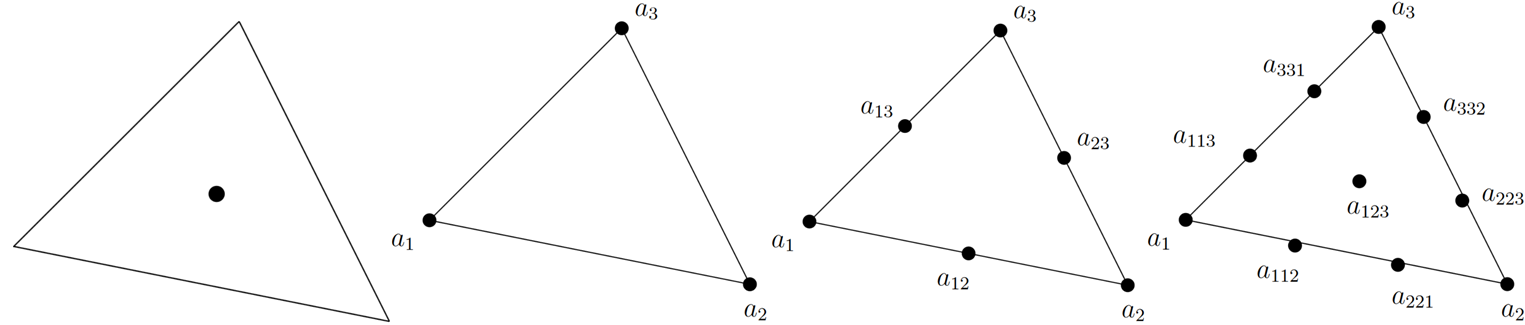
\includegraphics[width=1\textwidth]{./pics/FEM_Dreieck.png}
	\end{minipage}
	\begin{minipage}{0.49\textwidth}
		Quadrate:
		\begin{itemize}
			\item $Q_0$: stückweise konstantes FEM: $\dim(Q_0(K))=1$
			\item $Q_1$: konforme stückweise $d$-lineare FEM, $\dim(Q_1(K))=2^d\overset{d=2}{=}4$
			\item $Q_2$: konforme stückweise $d$-dimensionalen FEM, $\dim(Q_2(K))=3^d\overset{d=2}{=}8$
			\item $Q_3$: konforme stückweise $d$-kubische FEM, $\dim(Q_3(K))=4^d\overset{d=2}{=}16$.
		\end{itemize}
		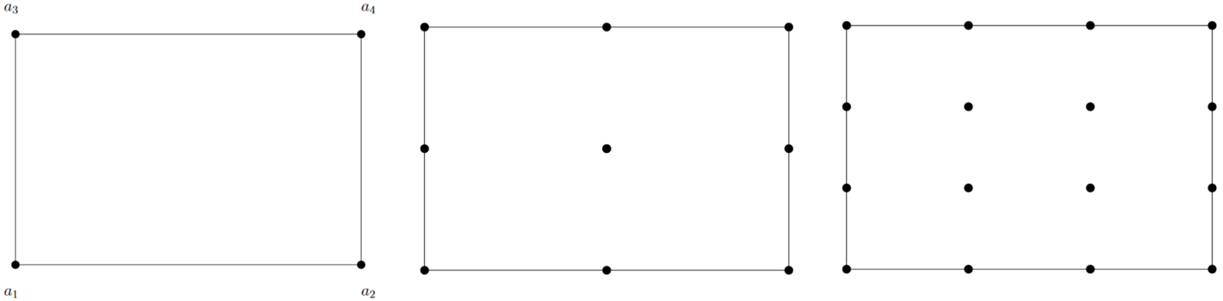
\includegraphics[width=1\textwidth]{./pics/FEM_Quadrat.png}
	\end{minipage}
	
	
	
\end{document}